
\providecommand{\hTwoCell}[5]{\tikz[baseline=-0.8ex]{%
  \node (rvl) at (0,0) {$#1$};
  \node (rvr) at (2.9,0) {$#2$};
  \draw[->] (rvl) to[bend left=28] node[above]{$\scriptstyle #3$} (rvr);
  \draw[->] (rvl) to[bend right=28] node[below]{$\scriptstyle #5$} (rvr);
  \node at (1.45,0) {$\scriptstyle #4$};}}

\section{右伴随右逆伴随}\label{sec:right-adjoint-right-inverse-adjunctions}

一类重要的\trAdjunction，是其\trCounit{}可逆的那些\trAdjunction。

\begin{definition}[右伴随右逆]\label{def:rajri}
2-\trCategory{}中的一支 1-\trCell{} $f\colon b\to a$ 容许一个%
\textbf{\trRightAdjoint\trRightInverse}，若它容许一个\trRightAdjoint{} $u\colon a\to b$
使得\trAdjunction{} $f\dashv u$ 的\trCounit{}是一个\trIsomorphism。在这种情形下，$f$ 是
$u$ 的\textbf{左伴随左逆}。
\end{definition}

余对偶则定义了带可逆单位的\textbf{\trLeftAdjoint\trRightInverse}或%
\textbf{右伴随左逆}（right adjoint left inverse）伴随类。

当 $f\dashv u$ 的\trCounit{}是一个\trIsomorphism{}时，其\trUnit{}的诸须状复合
$f\eta$ 与 $\eta u$ 也必是\trIsomorphism。事实上，要构造一个这种形式的\trAdjunction，
只需给出具有这些性质的诸 2-\trCell{}即可，正如下面这条 2-范畴引理所证明的那样。

\begin{lemma}\label{lem:rajri-modification}
设在 2-\trCategory{}中给定一对 1-\trCell{} $u\colon a\to b$ 与 $f\colon b\to a$，以及一
个 2-\trIsomorphism{} $fu\cong\mathrm{id}_{a}$。若存在 2-\trCell{}
$\eta'\colon\mathrm{id}_{b}\Rightarrow uf$ 使得 $f\eta'$ 与 $\eta'u$ 都是
2-\trIsomorphism，则 $f$ 左伴随于 $u$。此外，在 $u$ 是 $f$ 的\trSection{}这一特殊情形
下，$f$ 左伴随于 $u$，且该\trAdjunction{}的\trCounit{}为恒等。
\end{lemma}

由于 $f\eta'$ 与 $\eta'u$ 都是\trIsomorphism，而 $fu\cong\mathrm{id}_{a}$，第 2 章中的%
\cref{lem:minimal-adjunction-data}的那些「三角等式复合」便是可逆的，于是由该结果即可
得出 $f\dashv u$。事实上，从该证明中给出的构造可以看到，我们可以取所指定的同构
$fu\cong\mathrm{id}_{a}$ 来作这个\trAdjunction{}的\trCounit，因此特别地，当 $u$ 是 $f$
的\trSection{}时，这个\trCounit{}便可取为恒等。下面给出的直接证明便是把刚才概述的论证
加以展开。

\begin{proof}
设 $\epsilon\colon fu\Rightarrow\mathrm{id}_{a}$ 为此同构，在 $u$ 是 $f$ 的\trSection{}%
的情形下取它为恒等。我们将通过修改 $\eta'\colon\mathrm{id}_{b}\Rightarrow uf$ 来定义一
个以 $\epsilon$ 为\trCounit{}的\trAdjunction{} $f\dashv u$。「三角等式复合」
$\theta\coloneqq u\epsilon\cdot\eta'u\colon u\Rightarrow u$ 定义了 $u$ 的一个自同构。
定义
\[
\eta \coloneqq \mathrm{id}_{b} \xRightarrow{\;\eta'\;} uf
  \xRightarrow{\;\theta^{-1}f\;} uf
\coloneqq \mathrm{id}_{b} \xRightarrow{\;\eta'\;} uf
  \xRightarrow{\;(u\epsilon f)^{-1}\;} ufuf
  \xRightarrow{\;(\eta' uf)^{-1}\;} uf.
\]
立即可得 $u\epsilon\cdot\eta u=\mathrm{id}_{u}$，这由如下计算加以验证：
\begin{center}
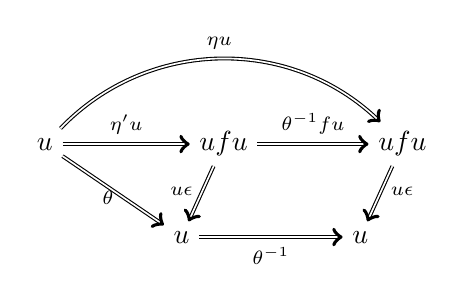
\begin{tikzpicture}[x=1.9em,y=1.4em]
  \node (u1)   at (0,1.2)    {$u$};
  \node (ufu1) at (3.4,1.2)  {$ufu$};
  \node (ufu2) at (6.8,1.2)  {$ufu$};
  \node (u2)   at (2.6,-1.2) {$u$};
  \node (u3)   at (6,-1.2)   {$u$};
  \draw[double,->] (u1) -- node[above]{$\scriptstyle\eta'u$} (ufu1);
  \draw[double,->] (ufu1) -- node[above]{$\scriptstyle\theta^{-1}fu$} (ufu2);
  \draw[double,->] (u1) to[bend left=45]
    node[above,pos=0.5]{$\scriptstyle\eta u$} (ufu2);
  \draw[double,->] (ufu1) -- node[left,pos=0.45]{$\scriptstyle u\epsilon$} (u2);
  \draw[double,->] (ufu2) -- node[right,pos=0.45]{$\scriptstyle u\epsilon$} (u3);
  \draw[double,->] (u1) -- node[left,pos=0.6]{$\scriptstyle\theta$} (u2);
  \draw[double,->] (u2) -- node[below]{$\scriptstyle\theta^{-1}$} (u3);
\end{tikzpicture}
\end{center}
另一个三角等式复合 $\phi\coloneqq\epsilon f\cdot f\eta$ 是一个\trIsomorphism——作为诸%
\trIsomorphism{}的复合——并且还是\trIdempotent：
\begin{center}
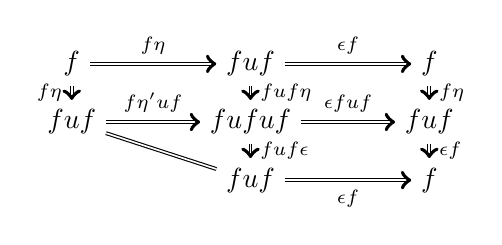
\begin{tikzpicture}[x=1.7em,y=1.4em]
  \node (f1)    at (0,1.5)     {$f$};
  \node (fuf1)  at (3.8,1.5)   {$fuf$};
  \node (f2)    at (7.6,1.5)   {$f$};
  \node (fuf2)  at (0,0)       {$fuf$};
  \node (fufuf) at (3.8,0)     {$fufuf$};
  \node (fuf3)  at (7.6,0)     {$fuf$};
  \node (fuf4)  at (3.8,-1.5)  {$fuf$};
  \node (f3)    at (7.6,-1.5)  {$f$};
  \draw[double,->] (f1) -- node[above]{$\scriptstyle f\eta$} (fuf1);
  \draw[double,->] (fuf1) -- node[above]{$\scriptstyle\epsilon f$} (f2);
  \draw[double,->] (f1) -- node[left]{$\scriptstyle f\eta$} (fuf2);
  \draw[double,->] (fuf1) -- node[right]{$\scriptstyle fuf\eta$} (fufuf);
  \draw[double,->] (fufuf) -- node[right]{$\scriptstyle fuf\epsilon$} (fuf4);
  \draw[double,->] (f2) -- node[right]{$\scriptstyle f\eta$} (fuf3);
  \draw[double,->] (fuf3) -- node[right]{$\scriptstyle\epsilon f$} (f3);
  \draw[double,->] (fuf2) -- node[above]{$\scriptstyle f\eta' uf$} (fufuf);
  \draw[double,->] (fufuf) -- node[above]{$\scriptstyle\epsilon fuf$} (fuf3);
  \draw[double,->] (fuf4) -- node[below]{$\scriptstyle\epsilon f$} (f3);
  \draw[double] (fuf2) -- (fuf4);
\end{tikzpicture}
\end{center}
由消去法，任何\trIdempotent{}同构都是恒等，这就证得
$\epsilon f\cdot f\eta=\mathrm{id}_{f}$。
\end{proof}

一个\trGeneralizedElement{} $y\colon z\to b$ 被称为属于一支 1-\trCell{}
$u\colon a\to b$ 的\textbf{本质像}（essential image），若存在一个\trGeneralizedElement{}
$x\colon z\to a$ 与一个可逆 2-\trCell{} $\beta\colon y\cong ux$。当\trFunctor{} $u$ 是
$f$ 的\trRightAdjoint\trRightInverse{}时，其本质像有一个便利的刻画：

\begin{lemma}\label{lem:rajri-essential-image}
一个\trGeneralizedElement{} $y\colon z\to b$ 属于\trRightAdjoint\trRightInverse{}
$u\colon a\to b$ 的本质像，当且仅当\trUnit{}分量 $\eta y\colon y\Rightarrow ufy$ 是一个%
\trIsomorphism。
\end{lemma}

\begin{proof}
尚需论证的只是：若给定一个可逆 2-\trCell{} $\beta\colon y\cong ux$，则\trUnit{}分量
$\eta y$ 也是一个\trIsomorphism。这由\cref{lem:naturality-of-whiskering}那条平凡的末尾
论断即得。从左下方那对可水平复合的 2-\trCell{}出发，\trWhiskering{}的自然性给出右下方
的交换图表：
\begin{center}
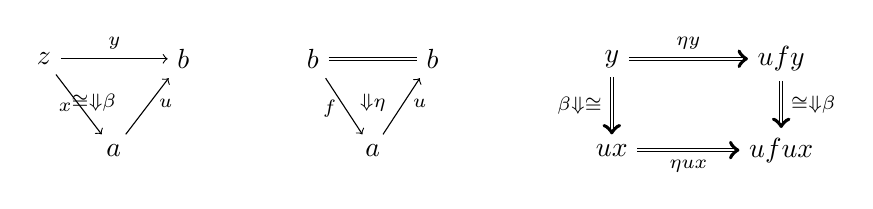
\begin{tikzpicture}[x=1.8em,y=1.5em]
  \node (z) at (0,1.1)    {$z$};
  \node (b) at (2.8,1.1)  {$b$};
  \node (a) at (1.4,-1.1) {$a$};
  \draw[->] (z) -- node[above]{$\scriptstyle y$} (b);
  \draw[->] (z) -- node[left,pos=0.55]{$\scriptstyle x$} (a);
  \draw[->] (a) -- node[right,pos=0.55]{$\scriptstyle u$} (b);
  \node at (1.0,0.05) {$\scriptstyle\cong\Downarrow\beta$};
  \node (b2) at (5.4,1.1)  {$b$};
  \node (b3) at (7.8,1.1)  {$b$};
  \node (a2) at (6.6,-1.1) {$a$};
  \draw[double] (b2) -- (b3);
  \draw[->] (b2) -- node[left,pos=0.55]{$\scriptstyle f$} (a2);
  \draw[->] (a2) -- node[right,pos=0.55]{$\scriptstyle u$} (b3);
  \node at (6.6,0.05) {$\scriptstyle\Downarrow\eta$};
  \node at (9.2,0) {$\rightsquigarrow$};
  \node (y)    at (11.4,1.1)  {$y$};
  \node (ufy)  at (14.8,1.1)  {$ufy$};
  \node (ux)   at (11.4,-1.1) {$ux$};
  \node (ufux) at (14.8,-1.1) {$ufux$};
  \draw[double,->] (y) -- node[above]{$\scriptstyle\eta y$} (ufy);
  \draw[double,->] (y) -- node[left]{$\scriptstyle\beta\Downarrow\cong$} (ux);
  \draw[double,->] (ufy) -- node[right]{$\scriptstyle\cong\Downarrow\beta$} (ufux);
  \draw[double,->] (ux) -- node[below]{$\scriptstyle\eta ux$} (ufux);
\end{tikzpicture}
\end{center}
由于 $u$ 是\trRightAdjoint\trRightInverse，$\eta u$ 可逆。于是，若 $\beta$ 可逆，则
$\eta y$ 亦可逆。
\end{proof}

有时，使用一种更严格的右伴随右逆伴随概念会更加方便，其中\trCounit{} $\epsilon$ 被要求
是恒等式 $fu=\mathrm{id}_{a}$。在这种情形下，由\trTriangleEqualities{}可得
$f\eta=\mathrm{id}_{f}$，从而\trUnit{}纤维化于 $a$ 之上。当\trLeftAdjoint{}在下述
2-范畴意义下是一个\trIsofibration{}时，同构意义下的右伴随右逆总可以替换为恒等意义下的
右伴随右逆（见第 3 章中的\cref{lem:rajri-fibered-adjunction}）。

\begin{definition}[等价纤维化]\label{def:rajri-isofibration}
2-\trCategory{}中的一支 1-\trCell{} $f\colon b\to a$ 定义一个%
\textbf{\trIsofibration}——此时该箭头通常记作「$\twoheadrightarrow$」——若给定任何
抵接于 $a$ 的可逆 2-\trCell{} $\alpha\colon fy\cong x$，连同其\trBoundary{} 1-\trCell{}%
之一穿过 $f$ 的一个指定提升，则存在抵接于 $b$ 的可逆 2-\trCell{}
$\beta\colon y\cong\bar{y}$ 带有这一\trBoundary{} 1-\trCell，它与 $f$ 须化后等于原先的
2-\trCell：
\begin{center}
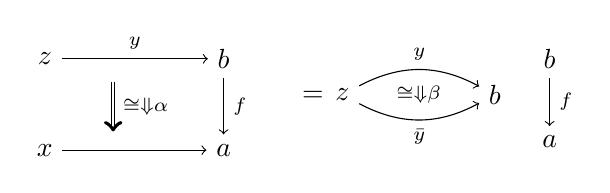
\begin{tikzpicture}[x=1.9em,y=1.5em]
  \node (z) at (0,0.9)    {$z$};
  \node (b) at (3.4,0.9)  {$b$};
  \node (xt) at (0,-1.3)  {$x$};
  \node (a) at (3.4,-1.3) {$a$};
  \draw[->] (z) -- node[above]{$\scriptstyle y$} (b);
  \draw[->] (b) -- node[right]{$\scriptstyle f$} (a);
  \draw[->] (xt) -- (a);
  \draw[double,->] (1.3,0.35) -- node[right]{$\scriptstyle\cong\Downarrow\alpha$}
    (1.3,-0.85);
  \node at (5.1,0) {$=$};
  \node at (7.1,0) {\hTwoCell{z}{b}{y}{\,\cong\Downarrow\beta\,}{\bar{y}}};
  \node (fb) at (9.6,0.9)  {$b$};
  \node (fa) at (9.6,-1.1) {$a$};
  \draw[->] (fb) -- node[right]{$\scriptstyle f$} (fa);
\end{tikzpicture}
\end{center}
\end{definition}

\begin{lemma}\label{lem:rajri-isofibration}
设 $f\colon b\twoheadrightarrow a$ 是 2-\trCategory{} $\mathcal{C}$ 中任何一支容许%
\trRightAdjoint{} $u'\colon a\to b$ 的\trIsofibration，其\trCounit{}
$\epsilon\colon fu'\cong\mathrm{id}_{a}$ 是一个\trIsomorphism。则 $u'$
\trIsomorphism{}于一个严格位于 $a$ 之上的\trFunctor{} $u$，后者定义了 $f$ 的一个严格右
伴随右逆，此时 $f\dashv u$ 在 2-\trCategory{} $\mathcal{C}_{/a}$——由以 $a$ 为余定义域
的\trIsofibration、$a$ 之上的交换三角形以及经须化后成为抵接于 $a$ 的恒等的
2-\trCell{}组成——中定义一个\trAdjunction。
\end{lemma}

\begin{center}
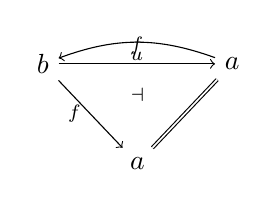
\begin{tikzpicture}[x=1.9em,y=1.5em]
  \node (b)  at (0,1.2)    {$b$};
  \node (a)  at (3.6,1.2)  {$a$};
  \node (a2) at (1.8,-1.2) {$a$};
  \draw[->] (b) -- node[above]{$\scriptstyle f$} (a);
  \draw[->] (a) to[bend right=20] node[below,pos=0.5]{$\scriptstyle u$} (b);
  \node at (1.8,0.45) {$\scriptstyle\dashv$};
  \draw[->] (b) -- node[left,pos=0.5]{$\scriptstyle f$} (a2);
  \draw[double] (a2) -- (a);
\end{tikzpicture}
\end{center}

\begin{proof}
将\trCounit{}同构经由\trIsofibration{} $f\colon b\twoheadrightarrow a$ 提升，由此定义
1-\trCell{} $u\colon a\to b$：
\begin{center}
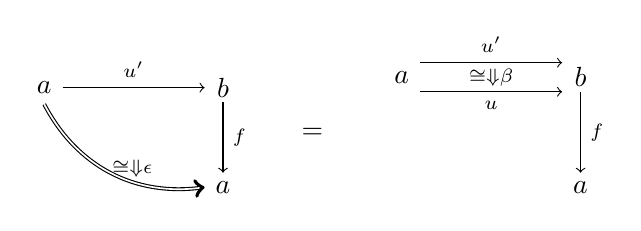
\begin{tikzpicture}[x=1.9em,y=1.5em]
  \node (la)  at (0,1.1)    {$a$};
  \node (lb)  at (3.4,1.1)  {$b$};
  \node (la2) at (3.4,-1.3) {$a$};
  \draw[->] (0.35,1.1) -- node[above]{$\scriptstyle u'$} (3.05,1.1);
  \draw[->] (3.4,0.75) -- node[right]{$\scriptstyle f$} (3.4,-0.95);
  \draw[double,->] (0,0.7) to[bend right=35]
    node[right,pos=0.45]{$\scriptstyle\cong\Downarrow\epsilon$} (3.05,-1.3);
  \node at (5.1,0) {$=$};
  \node (ra)  at (6.8,1.35)  {$a$};
  \node (rb)  at (10.2,1.35) {$b$};
  \node (ra2) at (10.2,-1.3) {$a$};
  \draw[->] (7.15,1.7) -- node[above]{$\scriptstyle u'$} (9.85,1.7);
  \draw[->] (7.15,1.0) -- node[below]{$\scriptstyle u$} (9.85,1.0);
  \node at (8.5,1.35) {$\scriptstyle\cong\Downarrow\beta$};
  \draw[->] (10.2,1.0) -- node[right]{$\scriptstyle f$} (10.2,-0.95);
\end{tikzpicture}
\end{center}
由构造即知 $fu=\mathrm{id}_{a}$，故 $u$ 定义了 $\mathcal{C}_{/a}$ 中的一个 1-\trCell。
由\trAdjunction{} $f\dashv u'$ 的\trTriangleEqualities，其\trUnit{}定义了一个
2-\trCell{} $\eta\colon\mathrm{id}_{b}\Rightarrow u'f$，其中 $\eta u'$ 与 $f\eta$ 均
可逆。复合 2-\trCell
\[
\eta' \coloneqq \mathrm{id}_{b} \xRightarrow{\;\eta\;} u'f
  \xRightarrow[\;\cong\;]{\;\beta f\;} uf
\]
位于 $\mathcal{C}_{/a}$ 中，且具有 $\eta'u$ 与 $f\eta$ 均可逆之性质。在 2-\trCategory{}
$\mathcal{C}_{/a}$ 中应用\cref{lem:rajri-modification}，这条 2-\trCell{}随后便可经修改
而定义一个\trAdjunction{} $f\dashv u$ 的\trUnit，其\trCounit{}满足 $fu=\mathrm{id}_{a}$。
\end{proof}

\subsection*{练习}

\begin{exercise}\label{ex:rajri-equivalent-adjunctions}
考虑一对等价的\trAdjunction，满足\cref{prop:equivalence-invariance-of-adjointness}的
条件。证明：若其中任一个是\trRightAdjoint\trRightInverse\trAdjunction，则二者皆是。
\end{exercise}

